%**************************************%
%* Generated from MathBook XML source *%
%*    on 2016-08-13T15:46:48-04:00    *%
%*                                    *%
%*   http://mathbook.pugetsound.edu   *%
%*                                    *%
%**************************************%
\documentclass[10pt,]{book}
%% Load geometry package to allow page margin adjustments
\usepackage{geometry}
\geometry{letterpaper,total={5.0in,9.0in}}
%% Custom Preamble Entries, early (use latex.preamble.early)
%% Inline math delimiters, \(, \), need to be robust
%% 2016-01-31:  latexrelease.sty  supersedes  fixltx2e.sty
%% If  latexrelease.sty  exists, bugfix is in kernel
%% If not, bugfix is in  fixltx2e.sty
%% See:  https://tug.org/TUGboat/tb36-3/tb114ltnews22.pdf
%% and read "Fewer fragile commands" in distribution's  latexchanges.pdf
\IfFileExists{latexrelease.sty}{}{\usepackage{fixltx2e}}
%% Page Layout Adjustments (latex.geometry)
%% This LaTeX file may be compiled with pdflatex, xelatex, or lualatex
%% The following provides engine-specific capabilities
%% Generally, xelatex and lualatex will do better languages other than US English
%% You can pick from the conditional if you will only ever use one engine
\usepackage{ifthen}
\usepackage{ifxetex,ifluatex}
\ifthenelse{\boolean{xetex} \or \boolean{luatex}}{%
%% begin: xelatex and lualatex-specific configuration
%% fontspec package will make Latin Modern (lmodern) the default font
\ifxetex\usepackage{xltxtra}\fi
\usepackage{fontspec}
%% realscripts is the only part of xltxtra relevant to lualatex 
\ifluatex\usepackage{realscripts}\fi
%% 
%% Extensive support for other languages
\usepackage{polyglossia}
\setdefaultlanguage{english}
%% Magyar (Hungarian)
\setotherlanguage{magyar}
%% Spanish
\setotherlanguage{spanish}
%% Vietnamese
\setotherlanguage{vietnamese}
%% end: xelatex and lualatex-specific configuration
}{%
%% begin: pdflatex-specific configuration
%% translate common Unicode to their LaTeX equivalents
%% Also, fontenc with T1 makes CM-Super the default font
%% (\input{ix-utf8enc.dfu} from the "inputenx" package is possible addition (broken?)
\usepackage[T1]{fontenc}
\usepackage[utf8]{inputenc}
%% end: pdflatex-specific configuration
}
%% Monospace font: Inconsolata (zi4)
%% Sponsored by TUG: http://levien.com/type/myfonts/inconsolata.html
%% See package documentation for excellent instructions
%% One caveat, seem to need full file name to locate OTF files
%% Loads the "upquote" package as needed, so we don't have to
%% Upright quotes might come from the  textcomp  package, which we also use
%% We employ the shapely \ell to match Google Font version
%% pdflatex: "varqu" option produces best upright quotes
%% xelatex,lualatex: add StylisticSet 1 for shapely \ell
%% xelatex,lualatex: add StylisticSet 2 for plain zero
%% xelatex,lualatex: we add StylisticSet 3 for upright quotes
%% 
\ifthenelse{\boolean{xetex} \or \boolean{luatex}}{%
%% begin: xelatex and lualatex-specific monospace font
\usepackage{zi4}
\setmonofont[BoldFont=Inconsolatazi4-Bold.otf,StylisticSet={1,3}]{Inconsolatazi4-Regular.otf}
%% end: xelatex and lualatex-specific monospace font
}{%
%% begin: pdflatex-specific monospace font
\usepackage[varqu]{zi4}
%% end: pdflatex-specific monospace font
}
%% Symbols, align environment, bracket-matrix
\usepackage{amsmath}
\usepackage{amssymb}
%% allow more columns to a matrix
%% can make this even bigger by overriding with  latex.preamble.late  processing option
\setcounter{MaxMatrixCols}{30}
%%
%% Color support, xcolor package
%% Always loaded.  Used for:
%% mdframed boxes, add/delete text, author tools
\PassOptionsToPackage{usenames,dvipsnames,svgnames,table}{xcolor}
\usepackage{xcolor}
%%
%% Semantic Macros
%% To preserve meaning in a LaTeX file
%% Only defined here if required in this document
%% Used for inline definitions of terms
\newcommand{\terminology}[1]{\textbf{#1}}
%% Subdivision Numbering, Chapters, Sections, Subsections, etc
%% Subdivision numbers may be turned off at some level ("depth")
%% A section *always* has depth 1, contrary to us counting from the document root
%% The latex default is 3.  If a larger number is present here, then
%% removing this command may make some cross-references ambiguous
%% The precursor variable $numbering-maxlevel is checked for consistency in the common XSL file
\setcounter{secnumdepth}{3}
%% Environments with amsthm package
%% Theorem-like environments in "plain" style, with or without proof
\usepackage{amsthm}
\theoremstyle{plain}
%% Numbering for Theorems, Conjectures, Examples, Figures, etc
%% Controlled by  numbering.theorems.level  processing parameter
%% Always need a theorem environment to set base numbering scheme
%% even if document has no theorems (but has other environments)
\newtheorem{theorem}{Theorem}[section]
%% Only variants actually used in document appear here
%% Style is like a theorem, and for statements without proofs
%% Numbering: all theorem-like numbered consecutively
%% i.e. Corollary 4.3 follows Theorem 4.2
%% Definition-like environments, normal text
%% Numbering is in sync with theorems, etc
\theoremstyle{definition}
\newtheorem{definition}[theorem]{Definition}
%% Remark-like environments, normal text
%% Numbering is in sync with theorems, etc
\theoremstyle{definition}
\newtheorem{note}[theorem]{Note}
%% Example-like environments, normal text
%% Numbering is in sync with theorems, etc
\theoremstyle{definition}
\newtheorem{example}[theorem]{Example}
%% Miscellaneous environments, normal text
%% Numbering for inline exercises and lists is in sync with theorems, etc
\theoremstyle{definition}
\newtheorem{exercise}[theorem]{Exercise}
%% Localize LaTeX supplied names (possibly none)
\renewcommand*{\proofname}{Proof}
\renewcommand*{\chaptername}{Chapter}
%% Equation Numbering
%% Controlled by  numbering.equations.level  processing parameter
\numberwithin{equation}{section}
%% For improved tables
\usepackage{array}
%% Some extra height on each row is desirable, especially with horizontal rules
%% Increment determined experimentally
\setlength{\extrarowheight}{0.2ex}
%% Define variable thickness horizontal rules, full and partial
%% Thicknesses are 0.03, 0.05, 0.08 in the  booktabs  package
\makeatletter
\newcommand{\hrulethin}  {\noalign{\hrule height 0.04em}}
\newcommand{\hrulemedium}{\noalign{\hrule height 0.07em}}
\newcommand{\hrulethick} {\noalign{\hrule height 0.11em}}
%% We preserve a copy of the \setlength package before other
%% packages (extpfeil) get a chance to load packages that redefine it
\let\oldsetlength\setlength
\newlength{\Oldarrayrulewidth}
\newcommand{\crulethin}[1]%
{\noalign{\global\oldsetlength{\Oldarrayrulewidth}{\arrayrulewidth}}%
\noalign{\global\oldsetlength{\arrayrulewidth}{0.04em}}\cline{#1}%
\noalign{\global\oldsetlength{\arrayrulewidth}{\Oldarrayrulewidth}}}%
\newcommand{\crulemedium}[1]%
{\noalign{\global\oldsetlength{\Oldarrayrulewidth}{\arrayrulewidth}}%
\noalign{\global\oldsetlength{\arrayrulewidth}{0.07em}}\cline{#1}%
\noalign{\global\oldsetlength{\arrayrulewidth}{\Oldarrayrulewidth}}}
\newcommand{\crulethick}[1]%
{\noalign{\global\oldsetlength{\Oldarrayrulewidth}{\arrayrulewidth}}%
\noalign{\global\oldsetlength{\arrayrulewidth}{0.11em}}\cline{#1}%
\noalign{\global\oldsetlength{\arrayrulewidth}{\Oldarrayrulewidth}}}
%% Single letter column specifiers defined via array package
\newcolumntype{A}{!{\vrule width 0.04em}}
\newcolumntype{B}{!{\vrule width 0.07em}}
\newcolumntype{C}{!{\vrule width 0.11em}}
\makeatother
%% Figures, Tables, Listings, Floats
%% The [H]ere option of the float package fixes floats in-place,
%% in deference to web usage, where floats are totally irrelevant
%% We re/define the figure, table and listing environments, if used
%%   1) New mbxfigure and/or mbxtable environments are defined with float package
%%   2) Standard LaTeX environments redefined to use new environments
%%   3) Standard LaTeX environments redefined to step theorem counter
%%   4) Counter for new environments is set to the theorem counter before caption
%% You can remove all this figure/table setup, to restore standard LaTeX behavior
%% HOWEVER, numbering of figures/tables AND theorems/examples/remarks, etc
%% WILL ALL de-synchronize with the numbering in the HTML version
%% You can remove the [H] argument of the \newfloat command, to allow flotation and 
%% preserve numbering, BUT the numbering may then appear "out-of-order"
\usepackage{float}
\usepackage[bf]{caption} % http://tex.stackexchange.com/questions/95631/defining-a-new-type-of-floating-environment 
\usepackage{newfloat}
% Figure environment setup so that it no longer floats
\SetupFloatingEnvironment{figure}{fileext=lof,placement={H},within=section,name=Figure}
% figures have the same number as theorems: http://tex.stackexchange.com/questions/16195/how-to-make-equations-figures-and-theorems-use-the-same-numbering-scheme 
\makeatletter
\let\c@figure\c@theorem
\makeatother
% Table environment setup so that it no longer floats
\SetupFloatingEnvironment{table}{fileext=lot,placement={H},within=section,name=Table}
% tables have the same number as theorems: http://tex.stackexchange.com/questions/16195/how-to-make-equations-figures-and-theorems-use-the-same-numbering-scheme 
\makeatletter
\let\c@table\c@theorem
\makeatother
%% Raster graphics inclusion, wrapped figures in paragraphs
%% \resizebox sometimes used for images in side-by-side layout
\usepackage{graphicx}
%%
%% Multiple column, column-major lists
\usepackage{multicol}
%% More flexible list management, esp. for references and exercises
%% But also for specifying labels (i.e. custom order) on nested lists
\usepackage{enumitem}
%% Lists of references in their own section, maximum depth 1
\newlist{referencelist}{description}{4}
\setlist[referencelist]{leftmargin=!,labelwidth=!,labelsep=0ex,itemsep=1.0ex,topsep=1.0ex,partopsep=0pt,parsep=0pt}
%% Lists of exercises in their own section, maximum depth 4
\newlist{exerciselist}{description}{4}
\setlist[exerciselist]{leftmargin=0pt,itemsep=1.0ex,topsep=1.0ex,partopsep=0pt,parsep=0pt}
%% Indented groups of exercises within an exercise section, maximum depth 4
\newlist{exercisegroup}{description}{4}
\setlist[exercisegroup]{leftmargin=2em,labelindent=2em,itemsep=1.0ex,topsep=1.0ex,partopsep=0pt,parsep=0pt}
%% Support for index creation
%% imakeidx package does not require extra pass (as with makeidx)
%% We set the title of the "Index" section via a keyword
%% And we provide language support for the "see" phrase
\usepackage{imakeidx}
\makeindex[title=Index, intoc=true]
\renewcommand{\seename}{see}
%% Package for tables spanning several pages
\usepackage{longtable}
%% hyperref driver does not need to be specified
\usepackage{hyperref}
%% configure hyperref's  \url  to match listings' inline verbatim
\renewcommand\UrlFont{\small\ttfamily}
%% Hyperlinking active in PDFs, all links solid and blue
\hypersetup{colorlinks=true,linkcolor=blue,citecolor=blue,filecolor=blue,urlcolor=blue}
\hypersetup{pdftitle={Applied Discrete Structures}}
%% If you manually remove hyperref, leave in this next command
\providecommand\phantomsection{}
%% If tikz has been loaded, replace ampersand with \amp macro
%% extpfeil package for certain extensible arrows,
%% as also provided by MathJax extension of the same name
%% NB: this package loads mtools, which loads calc, which redefines
%%     \setlength, so it can be removed if it seems to be in the 
%%     way and your math does not use:
%%     
%%     \xtwoheadrightarrow, \xtwoheadleftarrow, \xmapsto, \xlongequal, \xtofrom
%%     
%%     we have had to be extra careful with variable thickness
%%     lines in tables, and so also load this package late
\usepackage{extpfeil}
%% Custom Preamble Entries, late (use latex.preamble.late)
%% Begin: Author-provided macros
%% (From  docinfo/macros  element)
%% Plus three from MBX for XML characters
\newcommand{\identity}{\mathrm{id}}
\newcommand{\notdivide}{{\not{\mid}}}
\newcommand{\notsubset}{\not\subset}
\newcommand{\lcm}{\operatorname{lcm}}
\newcommand{\gf}{\operatorname{GF}}
\newcommand{\inn}{\operatorname{Inn}}
\newcommand{\aut}{\operatorname{Aut}}
\newcommand{\Hom}{\operatorname{Hom}}
\newcommand{\cis}{\operatorname{cis}}
\newcommand{\chr}{\operatorname{char}}
\newcommand{\Null}{\operatorname{Null}}
\newcommand{\lt}{ < }
\newcommand{\gt}{ > }
\newcommand{\amp}{ & }
%% End: Author-provided macros
%% Title page information for book
\title{Applied Discrete Structures}
\author{Al Doerr\\
Department of Mathematical Sciences\\
University of Massachusetts Lowell\\
\href{mailto:}{\nolinkurl{}}
\and
Ken Levasseur\\
Department of Mathematical Sciences\\
University of Massachusetts Lowell\\
\href{mailto:kenneth_levasseur@uml.edu}{\nolinkurl{kenneth_levasseur@uml.edu}}
}
\date{September, 2016}
\begin{document}
\frontmatter
%% begin: half-title
\thispagestyle{empty}
{\centering
\vspace*{0.28\textheight}
{\Huge Applied Discrete Structures}\\}
\clearpage
%% end:   half-title
%% begin: adcard
\thispagestyle{empty}
\null%
\clearpage
%% end:   adcard
%% begin: title page
%% Inspired by Peter Wilson's "titleDB" in "titlepages" CTAN package
\thispagestyle{empty}
{\centering
\vspace*{0.14\textheight}
{\Huge Applied Discrete Structures}\\[3\baselineskip]
{\Large Al Doerr}\\[0.5\baselineskip]
{\Large University of Massachusetts Lowell}\\[3\baselineskip]
{\Large Ken Levasseur}\\[0.5\baselineskip]
{\Large University of Massachusetts Lowell}\\[3\baselineskip]
{\Large September, 2016}\\}
\clearpage
%% end:   title page
%% begin: copyright-page
\thispagestyle{empty}
\vspace*{\stretch{2}}
\noindent\textcopyright\ 2016\quad{}Al Doerr, Ken Levasseur\\[0.5\baselineskip]
Applied Discrete Structures by Alan Doerr and Kenneth Levasseur is licensed under a Creative Commons Attribution-NonCommercial-ShareAlike 3.0 United States License. You are free to Share: copy and redistribute the material in any medium or format; Adapt: remix, transform, and build upon the material. You may not use the material for commercial purposes.  The licensor cannot revoke these freedoms as long as you follow the license terms.
			\par
\vspace*{\stretch{1}}
\null\clearpage
%% end:   copyright-page
%% begin: acknowledgement
\chapter*{Acknowledgements}\label{acknowledgement-1}
\addcontentsline{toc}{chapter}{Acknowledgements}
I would like to thank Rob Beezer, David Farmer and other participants on the \href{https://groups.google.com/forum/?fromgroups#!forum/mathbook-xml-support}{mathbook-xml-support group} for their guidance and work on MathBook XML.  Thanks to the Pedagogy Subcommittee of the UMass Lowell Transformational Education Committee for their financial assistance in helping getting this project started.%
%% end:   acknowledgement
%% begin: preface
\chapter*{Preface}\label{preface-1}
\addcontentsline{toc}{chapter}{Preface}
This version of \emph{Applied Discrete Structures} is being developed using \emph{Mathbook XML}, A lightweight XML application for authors of scientific articles, textbooks and monographs initiated by Rob Beezer, U. of Puget Sound.  %
\par
Sage (\href{http://sagemath.org}{sagemath.org}) is a free, open source, software system for advanced mathematics.  Sage can be used either on your own computer, a local server, or on SageMathCloud (\href{https://cloud.sagemath.com}{https://cloud.sagemath.com}). %
\par\hfill\begin{tabular}{l@{}}
Ken Levasseur\\
Lowell MA
\end{tabular}\\\par
%% end:   preface
%% begin: table of contents
\setcounter{tocdepth}{1}
\renewcommand*\contentsname{Contents}
\tableofcontents
%% end:   table of contents
\mainmatter
\typeout{************************************************}
\typeout{Chapter 1 Set Theory I}
\typeout{************************************************}
\chapter[Set Theory I]{Set Theory I}\label{chapter_5}
\typeout{************************************************}
\typeout{Introduction  Goals for Chapter 1}
\typeout{************************************************}
\section*{Goals for Chapter 1}
In this chapter we will cover some of the basic set language and notation that will be used throughout the text. Venn diagrams will be introduced in order to give the reader a clear picture of set operations. In addition, we will describe the binary representation of positive integers (Section 1.4) and introduce summation notation and its generalizations (Section 1.5).%
\typeout{************************************************}
\typeout{Section 1.1 Set Notation and Relations }
\typeout{************************************************}
\section[Set Notation and Relations ]{Set Notation and Relations }\label{Set-Notation-and-Relations}
\typeout{************************************************}
\typeout{Subsection 1.1.1 The notion of a set}
\typeout{************************************************}
\subsection[The notion of a set]{The notion of a set}\label{subsection-1}
The term set is intuitively understood by most people to mean a collection of objects that are called elements (of the set). This concept is the
starting point on which we will build more complex ideas, much as in-geometry where the concepts of point and line are left undefined. 
Because a set is such a simple notion, you may be surprised to learn that it is one of the most difficult concepts for mathematicians to define to
their own liking. For example, the description above is not a proper definition because it requires the definition of a collection. (How would you
define ``collection''?) Even deeper problems arise when you consider the possibility that a set could contain itself. Although these problems
are of real concern to some mathematicians, they will not be of any concern to us. 
Our first concern will be how to describe a set; that is, how do we most conveniently describe a set and the elements that are in it? If we are going to discuss a set for any length of time, we usually give it a name in the form of a capital letter (or occasionally some other symbol). In discussing set \( A\), if \( x\) is an element of \( A\), then we will write \(x \in  A\).\label{notation-1}
 On the other hand, if \( x\) is not an element
of \( A\), we write \(x \notin  A\).\label{notation-2}
 The most convenient way of describing the elements of a set will vary depending on the specific set. %
\par
\emph{ Enumeration.} When the elements of a set are enumerated (or listed) it is traditional to enclose them in braces. For example, the
set of binary digits is\(\{0, 1\}\) and the set of decimal digits is \(\{0, 1, 2, 3, 4, 5, 6, 7, 8, 9\}\). The choice of a name for these sets would
be arbitrary; but it would be ``logical'' to call them \( B\) and \( D\) , respectively. The choice of a set name is much like the
choice of an identifier name in programming. Some large sets can be enumerated without actually listing all the elements. For example, the letters
of the alphabet and the integers from 1 to 100 could be described as 
\(A = \{a, b, c,\ldots , x, y, z\}\), and \(G = \{1, 2, \ldots  , 99, 100\}\). 
The three consecutive ``dots'' are called an ellipsis. We use them when it is clear what elements are included but not listed. An ellipsis is
used in two other situations. To enumerate the positive integers, we would write \(\{1, 2, 3,\ldots  \}\), indicating that the list goes on infinitely.
If we want to list a more general set such as the integers between 1 and \( n\), where \( n\) is some undetermined positive integer, we
might write \(\{1,\ldots ,n\}\).
%
\par
\emph{ Standard Symbols}. Frequently used sets are usually given symbols that are reserved for them alone. For example, since we will be
referring to the positive integers throughout this book, we will use the symbol \(\mathbb{P}\) instead of writing \(\{1, 2, 3, \ldots \}\). A few
of the other sets of numbers that we will use frequently are: %
\par
\leavevmode%
\begin{itemize}[label=\textbullet]
\item{}\(\mathbb{(N)}\): the natural numbers, \(\{0, 1, 2, 3, \ldots \}\)%
\item{}\(\mathbb{(Z)}\): the integers, \(\{\ldots , -3, -2, -1, 0, 1, 2, 3,\ldots \}\)%
\item{}\(\mathbb{(Q)}\): the rational numbers%
\item{}\(\mathbb{(R)}\): the real numbers%
\item{}\(\mathbb{(C)}\): the complex numbers%
\end{itemize}
%
\par
\terminology{Set-Builder Notation}\index{Set-Builder Notation}. Another way of describing sets is to use set-builder notation. For example, we could define the rational numbers as \begin{equation*}\mathbb{Q}=\{a/b \mid a, b \in  \mathbb{Z}, b\neq 0\}\end{equation*}  Note that in the set-builder description for the rational numbers: %
\par
\leavevmode%
\begin{itemize}[label=\textbullet]
\item{} \(a/b\) indicates that a typical element of the set is a ``fraction.'' %
\item{} The vertical line, \(\mid\), is read ``such that'' or ``where,'' and is used interchangeably with a colon. %
\item{} \(a, b\in \mathbb{Z}\) is an abbreviated way of saying \(a\) and \(b\) are integers.  %
\item{} Commas in mathematics are read as ``and.'' %
\end{itemize}
%
\par
The important fact to keep in mind in set notation, or in any mathematical notation, is that it is meant to be a help, not a hindrance. We hope that notation will assist us in a more complete understanding of the collection of objects under consideration and will enable us to describe it in a concise manner. However, brevity of notation is not the aim of sets. If you prefer to write \(a\in \mathbb{Z}\) and \(b\in \mathbb{Z}\) instead of \(a, b\in \mathbb{Z}\), you should do so. Also, there are frequently many different, and equally good, ways of describing sets. For example, \(\left\{x\in
\mathbb{R} \mid x^{2}-5x+6=0\right\}\) and \(\left\{x \lvert  x\in \mathbb{R}, x^{2 }-5x+6=0\right\}\) both describe the solution set \(\{2, 3\}\). 
%
\par
A proper definition of the real numbers is beyond the scope of this text. It is sufficient to think of the real numbers as the set of points on a
number line. The complex numbers can be defined using set-builder notation as \(\mathbb{C} = \{a + b i:a, b \in \mathbb{R}\}\), where \(i^2 = -1\).  %
\par
In the following definition we will leave the word ``finite'' undefined.   
%
\begin{definition}[ Finite Set]\label{finite-set}
A set is a finite set if it has a finite number of elements. Any set that is not finite is an infinite set.%
\end{definition}
\begin{definition}[ Cardinality]\label{cardinality.}
\label{notation-3}
Let A be a finite set. The number of different elements in A is called its cardinality.%
\end{definition}
\par
As we will see later, there are different infinite cardinalities. We can't make this distinction until Chapter 7, so we will restrict cardinality to finite sets for now.%
\typeout{************************************************}
\typeout{Subsection 1.1.2 Subsets}
\typeout{************************************************}
\subsection[Subsets]{Subsets}\label{ss-subsets}
\begin{definition}[ Subset]\label{subset.}
\label{notation-4}
 Let \(A\) and \(B\) be sets. We say that \(A\) is a subset of \(B\)  if and only if every element of \(A\) is an element of \(B\). %
\end{definition}
\begin{example}[Some Subsets]\label{Some_Subsets}
\leavevmode%
\begin{enumerate}[label=\alph*]
\item\hypertarget{li-10}{} If \(A = \{3, 5, 8\}\) and \(B = \{5, 8, 3, 2, 6\}\), then \(A\subseteq B\). %
\item\hypertarget{li-11}{}  \(\mathbb{N}\subseteq \mathbb{Z}\subseteq \mathbb{Q}\subseteq \mathbb{R}\subseteq \mathbb{C}\) %
\item\hypertarget{li-12}{}If \(S = \{3, 5, 8\}\) and \(T = \{5, 3, 8\}\), then \(S \subseteq  T\) and \(T \subseteq  S\). %
\end{enumerate}
%
\end{example}
\begin{definition}[Set Equality]\label{set_equality}
Let \(A\) and \(B\) be sets. We say that \(A\) is equal to \(B\) (notation \(A = B\)) if and only if every element of
A is an element of B and conversely every element of B is an element of A; that is, \(A \subseteq  B\) and \(B \subseteq  A\).%
\end{definition}
\begin{example}[ Examples illustrating set equality]\label{set_equality_examples}
\leavevmode%
\begin{enumerate}[label=\alph*]
\item\hypertarget{li-13}{}In \hyperref[Some_Subsets]{Example~\ref{Some_Subsets}}, \(S = T\). Note that the ordering of the elements is unimportant. %
\item\hypertarget{li-14}{}The number of times that an element appears in an enumeration doesn't affect a set. For example, if \(A = \{1, 5, 3, 5\}\) and \(B = \{1, 5, 3\}\), then \(A = B\).  Warning to readers of other texts: Some books introduce the concept of a multiset, in which the number of occurrences of an element matters.%
\end{enumerate}
%
\end{example}
A few comments are in order about the expression ``if and only if'' as used in our definitions. This expression means ``is equivalent to saying,''
or more exactly, that the word (or concept) being defined can at any time be replaced by the defining expression. Conversely, the expression that
defines the word (or concept) can be replaced by the word. %
\par
Occasionally there is need to discuss the set that contains no elements, namely the empty set, which is denoted by \(\emptyset\)\label{notation-5}
\index{Empty set}.
This set is also called the null set.%
\par
It is clear, we hope, from the definition of a subset, that given any set \( A\) we have \(A\subseteq A\) and \(\emptyset \subseteq A\). If \(A\) is nonempty, then 
 \(A\) is called an \terminology{improper subset}\index{Improper subset} of \(A\).  All other subsets of \(A\), including the empty set, are called \terminology{proper subsets }\index{Proper subset} of \(A\). %
\begin{note}[]\label{note-1}
Not everyone is in agreement on whether the empty set is a proper subset of any set.  In fact earlier editions of this book sided with those who considered the empty set an improper subset.  However, we bow to the emerging consensus at this time.%
\end{note}
\typeout{************************************************}
\typeout{Exercises 1.1.3 Exercises for Section 1.1 }
\typeout{************************************************}
\subsection[Exercises for Section 1.1 ]{Exercises for Section 1.1 }\label{exercises-1}
\hypertarget{exercisegroup-1}{}\typeout{************************************************}
\typeout{Introduction  }
\typeout{************************************************}
A Exercises%
\begin{exercisegroup}
\item[1.]\hypertarget{exercise-1}{}List four elements of each of the following sets:%
\par
\leavevmode%
\begin{enumerate}[label=\alph*]
\item\hypertarget{li-15}{} \(\{k \in  \mathbb{P} \mid {k - 1} \textrm{ is a multiple of 7}\}\) %
\item\hypertarget{li-16}{} \(\{x \mid x \textrm{ is a fruit and its skin is normally eaten }\}\)%
\item\hypertarget{li-17}{}\(\{x \in \mathbb{Q}\mid \frac{1}{x} \in \mathbb{Z}\}\)%
\item\hypertarget{li-18}{} \(\{2n \mid n \in \mathbb{Z}, n < 0 \}\)%
\item\hypertarget{li-19}{} \(\{s \mid s = 1 + 2 + \cdots  + n, n \in \mathbb{P}\}\)%
\end{enumerate}
%
\par\smallskip
\par\smallskip
\noindent\textbf{Answer.}\hypertarget{answer-1}{}\quad
These answers are not unique.%
\par
\leavevmode%
\begin{multicols}{3}
\begin{enumerate}[label=\alph*]
\item\hypertarget{li-20}{} \(8, 15, 22, 29\)%
\item\hypertarget{li-21}{} apple, pear, peach, plum %
\item\hypertarget{li-22}{} \(1/2, 1/3, 1/4, 1/5\)%
\item\hypertarget{li-23}{} \(-8, -6, -4, -2\)%
\item\hypertarget{li-24}{}\(6, 10, 15, 21\)%
\end{enumerate}
\end{multicols}
%
\item[2.]\hypertarget{exercise-2}{} List all elements of the following sets:%
\par
\leavevmode%
\begin{enumerate}[label=\alph*]
\item\hypertarget{li-25}{} \(\{\frac{1}{n} \mid n \in \{3,4,5,6\}\}\)%
\item\hypertarget{li-26}{}  \(\{\alpha \in  \textrm{ the alphabet } \mid  \alpha \textrm{ precedes F}\}\)%
\item\hypertarget{li-27}{} \(\{-k \mid k \in \mathbb{P}\}\)%
\item\hypertarget{li-28}{} \(\{n^2 \mid  n = -2, -1, 0, 1, 2\}\)%
\item\hypertarget{li-29}{} \(\{n \in  \mathbb{P} \mid n \textrm{is a  factor of  24 }\}\)%
\end{enumerate}
%
\par\smallskip
\item[3.]\hypertarget{exercise-3}{}  Describe the following sets using set-builder notation. %
\par
\leavevmode%
\begin{multicols}{1}
\begin{enumerate}[label=\alph*]
\item\hypertarget{li-30}{} \(\{ 5, 7, 9, \dots , 77, 79\}\) %
\item\hypertarget{li-31}{}the rational numbers that are strictly between \(-1\) and \(1\) %
\item\hypertarget{li-32}{} the even integers%
\item\hypertarget{li-33}{} \(\{-18, -9,0,9, 18,27, \dots \}\) %
\end{enumerate}
\end{multicols}
%
\par\smallskip
\par\smallskip
\noindent\textbf{Answer.}\hypertarget{answer-2}{}\quad
\leavevmode%
\begin{enumerate}[label=\alph*]
\item\hypertarget{li-34}{} \(\{2k + 1 \mid k \in  \mathbb{Z}, 2 \leqslant  k \leqslant  39\}\) %
\item\hypertarget{li-35}{} \(\{x \in \mathbb{Q}\mid  -1 < x < 1\}\)%
\item\hypertarget{li-36}{} \(\{2n\mid n \in  \mathbb{Z}\}\) %
\item\hypertarget{li-37}{} \(\{9n\mid n \in \mathbb{Z}, -2 \leq  n\}\)%
\end{enumerate}
%
\item[4.]\hypertarget{exercise-4}{}  Use set-builder notation to describe the following sets: %
\par
\leavevmode%
\begin{multicols}{1}
\begin{enumerate}[label=\alph*]
\item\hypertarget{li-38}{}\(\{1, 2, 3, 4, 5, 6, 7\}\) %
\item\hypertarget{li-39}{} \(\{1, 10, 100, 1000, 10000\}\)  %
\item\hypertarget{li-40}{} \(\{1, 1/2, 1/3, 1/4, 1/5, . . .\}\) %
\item\hypertarget{li-41}{}  \(\{0\}\)%
\end{enumerate}
\end{multicols}
%
\par\smallskip
\item[5.]\hypertarget{exercise-5}{}  Let \(A = \{0, 2, 3\}\), \(B = \{2, 3\}\), and \(C = \{1, 5, 9\}\). Determine which of the following statements are true. Give reasons for
your answers. %
\par
\leavevmode%
\begin{multicols}{2}
\begin{enumerate}[label=\alph*]
\item\hypertarget{li-42}{}\(3 \in  A\)%
\item\hypertarget{li-43}{}\(\{3\} \in  A\) %
\item\hypertarget{li-44}{}\(\{3\} \subseteq A\)%
\item\hypertarget{li-45}{} \(B\subseteq A\)%
\item\hypertarget{li-46}{} \(A\subseteq B\)%
\item\hypertarget{li-47}{}\(\emptyset \subseteq C\) %
\item\hypertarget{li-48}{} \(\emptyset \in A\)%
\item\hypertarget{li-49}{} \(A\subseteq A\)%
\end{enumerate}
\end{multicols}
%
\par\smallskip
\par\smallskip
\noindent\textbf{Answer.}\hypertarget{answer-3}{}\quad
\leavevmode%
\begin{multicols}{3}
\begin{enumerate}[label=\alph*]
\item\hypertarget{li-50}{} True%
\item\hypertarget{li-51}{} False%
\item\hypertarget{li-52}{} True%
\item\hypertarget{li-53}{} True%
\item\hypertarget{li-54}{} False%
\item\hypertarget{li-55}{}True%
\item\hypertarget{li-56}{} False%
\item\hypertarget{li-57}{} True%
\end{enumerate}
\end{multicols}
%
\end{exercisegroup}
\par\smallskip\noindent
\hypertarget{exercisegroup-2}{}\typeout{************************************************}
\typeout{Introduction  }
\typeout{************************************************}
C Exercises%
\begin{exercisegroup}
\item[6.]\hypertarget{exercise-6}{} One reason that we left the definition of a set vague is Russell's Paradox. Many mathematics and logic books contain an account of this paradox. Two references are Stoll and Quine. Find one such reference and read it.  %
\par\smallskip
\end{exercisegroup}
\par\smallskip\noindent
\typeout{************************************************}
\typeout{Section 1.2 Generating Functions}
\typeout{************************************************}
\section[Generating Functions]{Generating Functions}\label{s-generating-functions}
\index{Generating Functions}\typeout{************************************************}
\typeout{Introduction  }
\typeout{************************************************}
This section contains an introduction to the topic of generating functions and how they are used to solve recurrence relations, among other problems.
Methods that employ generating functions are based on the concept that you can take a problem involving sequences and translate it into a problem
involving generating functions. Once you've solved the new problem, a translation back to sequences gives you a solution of the original problem.%
\par
This section covers:%
\par
\leavevmode%
\begin{enumerate}[label=\arabic*]
\item\hypertarget{li-58}{}The definition of a generating function;%
\item\hypertarget{li-59}{}Solution of a recurrence relation using generating functions to identify the skills needed to use generating functions;\\%
\item\hypertarget{li-60}{}An introduction and/or review of the skills identified in point b;\\%
\item\hypertarget{li-61}{}Some applications of generating functions.%
\end{enumerate}
%
\typeout{************************************************}
\typeout{Subsection 1.2.1 Definition}
\typeout{************************************************}
\subsection[Definition]{Definition}\label{ss-what-is-a-generating-function}
\begin{definition}[Generating Function of a Sequence]\label{def-generating-function}
\index{Generating Function}\label{notation-6}
The generating function of a sequence S with terms \(S_0,S_1 ,S_2, \dots \),  is the infinite sum
 \[G(S;z)=\sum_{n=0}^{\infty} S_n z^n=S_0+S_1 z+S_2 z^2+S_3 z^3+\cdots\]
The domain and codomain of generating functions will not be of any concern to us since we will only be performing algebraic operations on them.%
\end{definition}
\begin{example}[First Examples]\label{ex-first-gf-examples}
\leavevmode%
\begin{enumerate}[label=\alph*]
\item\hypertarget{li-62}{} If \(S_n = 3^n\),\(n \geq  0\), then

\(G(S;z) = 1 + 3z + 9z^2 + 27z^3 +\cdots \\
\\
\quad =\sum_{n=0}^{\infty} 3^n z^n\\
\\
\quad =\sum_{n=0}^{\infty} (3 z)^n\)

We can get a closed form expression for \(G(S;z)\) by observing that \(G(S;z) - 3z G(S;z) = 1\). Therefore,

\(G(S;z) =\frac{1}{1-3 z}\).%
\item\hypertarget{li-63}{}Finite sequences have generating functions. For example, the sequence of binomial coefficients \(C(n; 0)\), \(C(n; 1)\), \(\ldots\),\(C(n;
n)\), \(n \geq  1\) has generating function

\(G(C(n; \cdot ); z) = C(n; 0) + C(n; 1)z +\cdots  + C(n; n)z^n\\
\\
\quad \quad = \sum_{k=0}^{\infty} C(n;k) z^k\\
\\
\quad \quad =(1+z)^n\)

by application of the binomial formula.%
\item\hypertarget{li-64}{} If \(Q(n) = n^2\),

\(G(Q;z)=\sum_{n=0}^{\infty} n^2 z^n=\sum_{k=0}^{\infty} k^2 z^k\)

Note that the index that is used in the summation has no significance. Also, note that the lower limit of the summation could start at 1 since \(Q(0)=0\).%
\end{enumerate}
%
\end{example}
\typeout{************************************************}
\typeout{Subsection 1.2.2 Solution of a Recurrence Relation Using Generating Functions}
\typeout{************************************************}
\subsection[Solution of a Recurrence Relation Using Generating Functions]{Solution of a Recurrence Relation Using Generating Functions}\label{ss-solution-of-rr-using-generating-functions}
We illustrate the use of generating functions by solving
 \(S(n) - 2S(n - 1) - 3S(n - 2) = 0\), \(n \geq  2\), with \(S(0) = 3\) and \(S(1) = 1\).%
\par
\leavevmode%
\begin{enumerate}[label=\arabic*]
\item\hypertarget{li-65}{} Translate the recurrence relation into an equation about generating functions.%
\par
Let \(V(n) = S(n) - 2S (n - 1) - 3S (n - 2)\), \(n \geq  2\), with \(V(0) = 0\) and \(V(1) = 0\). Therefore,
\[G(V;z) = 0 + 0z +\sum_{n=2}^{\infty}  (S(n) - 2S (n - 1) - 3S (n - 2)) z^n= 0\]
%
\item\hypertarget{li-66}{}Solve for the generating function of the unknown sequence,\(G(S,z) = \sum_{n=0}^{\infty} S_n z^n\).
 \begin{equation*}
 \begin{split}
 0 & =\sum_{n=2}^{\infty}  (S(n) - 2S (n - 1) - 3S (n - 2)) z^n\\
 	& =\sum_{n=2}^{\infty} S(n) z^n-2 (\sum_{n=2}^{\infty
} S(n-1) z^n)-3(\sum_{n=2}^{\infty} S(n-2) z^n)
\end{split}
\end{equation*}
%
\par
Close examination of the three sums above shows:%
\par
%
\begin{enumerate}[label=\alph*]
\item\hypertarget{li-67}{}
\begin{equation*}
\begin{split}
\sum_{n=2}^{\infty} S_n z^n &=\sum_{n=0}^{\infty} S_n z^n - S(0)-S(1)z\\
			&= G(S;z)-3-z\\
\end{split}
\end{equation*}
since \(S(0)=3\) and \(S(1)=1\).%
\item\hypertarget{li-68}{}
\begin{equation*}
\begin{split}
\sum_{n=2}^{\infty} S(n-1) z^n &=z(\sum_{n=2}^{\infty} S(n-1) z^{n-1})\\
		& =z(\sum_{n=1}^{\infty} S(n) z^n)\\
		& = z(\sum_{n=0}^{\infty} S(n) z^n-S(0))\\
		&= z(G(S;z)-3\\\
\end{split}
\end{equation*}
%
\item\hypertarget{li-69}{}
\begin{equation*}
\begin{split}
\sum_{n=2}^{\infty} S(n-2) z^n  & = z^2(\sum_{n=2}^{\infty} S(n-2) z^{n-2})\\
	& =z^2G(S;z)\\
\end{split}
\end{equation*}
%
\par
Therefore, 
\begin{equation*}
\begin{split}
&(G(S;z)-3-z)-2z(G(S;z)-3)-3z^2G(S;z)=0\\
	 & \Rightarrow G(S;z)-2z G(S;z)-3z^2G(S;z)=3 - 5z\\
		&\Rightarrow G(S;z)=\frac{3-5z}{1-2z-3z^2}\\
\end{split}
\end{equation*}
%
\end{enumerate}
%
\item\hypertarget{li-70}{}Determine the sequence whose generating function is the one we got in Step 2.%
\par
For our example, we need to know one general fact about the closed form expression of an exponential sequence (a proof will be given later):
\begin{gather}
T(n)=b a^n ,n\geq 0 \Leftrightarrow G(T;z)=\frac{b}{1-a z} \label{gf-of-exp}
\end{gather}
%
\par
Now, in order to recognize \(S\) in our example, we must write our closed form expression for \(G(S;z)\) as a sum of terms like \(G(T;z)\) above. Note that the denominator of \(G(S;z)\) can be factored:

 \[G(S;z)=\frac{3-5z}{1-2z-3z^2} =\frac{3-5z}{(1-3z)(1+z)}\]

If you look at this last expression for \(G(S;z)\) closely, you can imagine how it could be the result of addition of two fractions,
\begin{gather}
\frac{3-5z}{(1-3z)(1+z)} = \frac{A}{1-3z}+ \frac{B}{1+z}
\label{eq-pf}
\end{gather}
where \(A\) and \(B\) are two real numbers that must be determined. Starting on the right of \hyperref[eq-pf]{(\ref{eq-pf})}, it should be clear that the sum, for
any \(A\) and \(B\), would look like the left-hand side. The process of finding values of \(A\) and \(B\) that make \hyperref[eq-pf]{(\ref{eq-pf})}
true is called the \terminology{partial fractions decomposition} of the left-hand side:

\begin{equation*}
\begin{split}
\frac{A}{1-3z}+ \frac{B}{1+z} &=\frac{A(1+z)}{(1-3z)(1+z)}+ \frac{B(1-3z)}{(1-3z)(1+z)}\\
		& =\frac{(A+B)+(A-3B)z}{(1-3z)(1+z)}\\
\end{split}
\end{equation*}
%
\par
Therefore,



 \[\left\{
\begin{array}{c}
 A+B=3 \\
 A-3B=-5 \\
\end{array}
\right\}\Rightarrow \left\{
\begin{array}{c}
 A=1 \\
 B=2 \\
\end{array}
\right\}\]
and

\[G(S;z)= \frac{1}{1-3z}+ \frac{2}{1+z}\]

%
\par
We can apply \hyperref[gf-of-exp]{(\ref{gf-of-exp})} to each term of G(S;z):%
\par
%
\begin{itemize}[label=\textbullet]
\item{}\(\frac{1}{1-3z}\) is the generating function for \(S_1(n)=1\cdot  3^n= 3^n\)%
\item{}\(\frac{2}{1+z}\) is the generating function for \(S_2(n)=2(-1)^n\).%
\end{itemize}
%
\par
Therefore, \(S(n)=3^n+ 2(-1)^n\).%
\end{enumerate}
%
\par
From this example, we see that there are several skills that must be mastered in order to work with generating functions. You must be able to:%
\par
\leavevmode%
\begin{enumerate}[label=\alph*]
\item\hypertarget{li-73}{}Manipulate summation expressions and their indices (in Step 2).%
\item\hypertarget{li-74}{}Solve algebraic equations and manipulate algebraic expressions, including partial function decompositions (Steps 2 and 3).%
\item\hypertarget{li-75}{} Identify sequences with their generating functions (Steps 1 and 3).%
\end{enumerate}
%
\par
We will concentrate on the last skill first, a proficiency in the other skills is a product of doing as many exercises and reading as many examples as possible.%
\par
First, we will identify the operations on sequences and on generating functions.%
\typeout{************************************************}
\typeout{Subsection 1.2.3 Operations on Sequences}
\typeout{************************************************}
\subsection[Operations on Sequences]{Operations on Sequences}\label{ops-on-sequences}
\begin{definition}[Operations on Sequences]\label{definition-6}
\index{Sequences!Operations on,}\label{notation-7}
\label{notation-8}
\label{notation-9}
Let \(S\) and \(T\) be sequences of numbers and let \(c\) be a real number. Define the sum \(S + T\), the scalar product \(c S\), the product \(S T\), the convolution \(S*T\), the pop operation \(S\uparrow\) (read ``S pop''), and the push
operation \(S\downarrow\) (read ``S push'') term-wise for \(k \geq  0\) by
\begin{align}
(S + T)(k) = S(k) + T(k)\label{seq-op-add}\\
(c S)(k) = c S(k)\label{seq-op-sc-mult}\\
(S \cdot T)(k) = S(k)T(k)\)\label{seq-op-mult}\\
(S*T)(k) = \sum_{j=0}^k S(j) T(k-j)\)\label{seq-op-convolve}\\
(S\uparrow )(k) = S(k+1)\)\label{seq-op-pop}\\
(S\downarrow )(k)=\left\{\begin{array}{cc} 0 & \textrm{ if } k=0 \\ S(k-1) & \textrm{ if } k>0 \\\end{array}\)\\
\end{array}\label{seq-op-push}
\end{align}%
\end{definition}
If one imagines a sequence to be a matrix with one row and an infinite number of columns, \(S + T\) and \(c S\) are exactly as in matrix addition
and scalar multiplication. There is no obvious similarity between the other operations and matrix operations.%
\par
The pop and push operations can be understood by imagining a sequence to be an infinite stack of numbers with \(S(0)\) at the top, \(S(1)\) next,
etc., as in \hyperref[fig-pop-push]{Figure~\ref{fig-pop-push}}a. The sequence \(S\uparrow\) is obtained by ``popping'' S(0) from the stack, leaving a stack as in \hyperref[fig-pop-push]{Figure~\ref{fig-pop-push}}b, with
S(1) at the top, S(2) next, etc. The sequence S I is obtained by placing a zero at the top of the stack, resulting in a stack as in \hyperref[fig-pop-push]{Figure~\ref{fig-pop-push}}c.
Keep these figures in mind when we discuss the pop and push operations.%
\leavevmode%
\begin{figure}
\centering
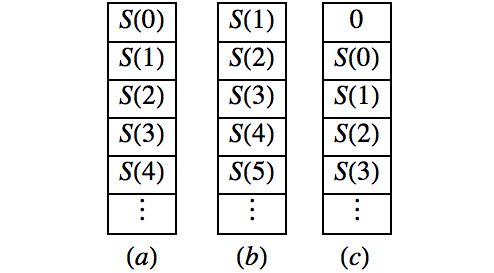
\includegraphics[width=1\linewidth]{images/fig-pop-push.png}
\caption{Stack interpretation of pop and push operation\label{fig-pop-push}}
\end{figure}
\begin{example}[Some Sequence Operations]\label{ex-some-sequence-operations}
If \(S(n) = n\), \(T(n) = n^2\), \(U(n) = 2^n\), and \(R(n) =n 2^n\) %
\par
\leavevmode%
\begin{enumerate}[label=\alph*]
\item\hypertarget{li-76}{} \((S + T)(n) = n + n^2\)%
\item\hypertarget{li-77}{}\((U + R)(n) = 2^n+ n 2^n= (1+n)2^n\)%
\item\hypertarget{li-78}{}\((2 U)(n) = 2\cdot 2^n= 2^{n+1}\)%
\item\hypertarget{li-79}{} \((\frac{1}{2}R)(n)= \frac{1}{2}n 2^n= n 2^{n-1}\)%
\item\hypertarget{li-80}{} \((S\cdot T)(n) = n n^2 = n^3\)%
\item\hypertarget{li-81}{}\((S*T)(n)= \sum_{j=0}^n S(j) T(n-j)= \sum_{j=0}^n j (n-j)^2\\
\\
\quad \quad =\sum_{j=0}^n ( j n^2-2 n j^2 + j^3)\\
\\
\quad \quad = n^2\sum_{j=0}^n j-2n \sum_{j=0}^n j^2 + \sum_{j=0}^n j ^3\\
\\
\quad \quad =n^{2 }(\frac{n (n+1)}{2})- 2n(\frac{(2n+1)(n+1)n}{6})+\frac{1}{4} n^2 (n+1)^2\\
\\
\quad \quad = \frac{n^2(n+1)(n-1)}{12}\)%
\item\hypertarget{li-82}{}\((U*U)(n) =\sum_{j=0}^n U(j) U(n-j)\\
\\
\quad \quad =\sum_{j=0}^n 2^j 2^{n-j}\\
\\
\quad \quad = (n+1)2^n\)%
\item\hypertarget{li-83}{} \((S\uparrow )(n)=n+1\)%
\item\hypertarget{li-84}{}\((S\downarrow )(n)=\max (0,n-1)\)%
\item\hypertarget{li-85}{} \(((S\downarrow )\downarrow )(n)= \max (0, n - 2)\)%
\item\hypertarget{li-86}{} \((U\downarrow )(n)=\left\{
\begin{array}{cc}
 2^{n-1} & \textrm{ if } n>0 \\
 0 & \textrm{ if } n=0 \\
\end{array}
\)%
\item\hypertarget{li-87}{} \(((U\downarrow )\uparrow )(n)=(U\downarrow )(n+1)= 2^n= U(n)\)%
\item\hypertarget{li-88}{} \(((U\uparrow )\downarrow ) (n)=\left\{
\begin{array}{cc}
 0 & \textrm{ if } n = 0 \\
 U(n) & \textrm{ if } n>0 \\
\end{array}
\)%
\end{enumerate}
%
\end{example}
\par
Note that \((U\downarrow )\uparrow \neq (U\uparrow )\downarrow\).%
\begin{definition}[ Multiple Pop and Push]\label{def-multiple-pop-and-push}
\index{Multiple Pop and Push:}\label{notation-10}
\label{notation-11}
If S is a sequence of numbers and \(p\) a positive integer greater than 1, define
\[S\uparrow p = (S\uparrow (p - 1))\uparrow\textrm{ if }p \geq  2 \textrm{ and }S\uparrow 1 = S\uparrow\] 
Similarly, define
\[S\downarrow p = (S\downarrow (p - 1))\downarrow\)\textrm{ if }\(p \geq  2\textrm{ and }S\downarrow 1 = S\downarrow\]
%
\end{definition}
\par
In general, \(S \uparrow p)(k) = S(k+p),\) and



\begin{equation*}
(S\downarrow p)(k)=\left\{
   \begin{array}{cc}
 0 & \textrm{ if } k < p \\
 S(k-p) & \textrm{ if } k\geq p \\
\end{array}

\end{equation*}
%
\typeout{************************************************}
\typeout{Subsection 1.2.4 Operations on Generating Functions}
\typeout{************************************************}
\subsection[Operations on Generating Functions]{Operations on Generating Functions}\label{sss-operations-on-generating-functions}
\index{Generating Functions!Operations on,}\begin{definition}[Operations on Generating Functions]\label{definition-8}
\index{Generating Functions!Operations on,}If  \(G(z)=\sum_{k=0}^{\infty} a_k z^k\) and \(H(z) =\sum_{k=0}^{\infty} b_k z^k\)
are generating functions and \(c\) is a real number, then the sum \(G + H\), scalar product \(c G\), product \(G H\), and monomial product \(z^p G\), \(p \geq  1\) are generating functions, where

\begin{gather}
(G + H)(z)=\sum_{k=0}^{\infty} (a_k+b_k) z^k\label{gf-sum}\\
[(c G)(z)=\sum_{k=0}^{\infty} c a_k z^k\label{gf-scalarmult}\\
(G H)(z) = \sum_{k=0}^{\infty} c z^k \textrm{ where } c_k= \sum_{j=0}^k a_jb_{k-j}\label{gf-product}\\
(z^p G)(z) = z^p\sum_{k=0}^{\infty} a_k z^k=\sum_{k=0}^{\infty} a_k z^{k+p} = \sum_{n=p}^{\infty} a_{n-p} z^n\label{gf-shift}
\end{gather}
%
\par
The last sum is obtained by substituting \(n - p\) for \(k\) in the previous sum.%
\end{definition}
\begin{example}[Some operations on generating functions]\label{ex-some-gf-operations}
If

\(D(z) =\sum_{k=0}^{\infty} kz^k\) and \(H(z) =\sum_{k=0}^{\infty} 2^k z^k\) 

then

\((D + H)(z) =\sum_{k=0}^{\infty} (k+2^k) z^k\) 

\((2H)(z)= \sum_{k=0}^{\infty} 2\cdot 2^kz^k =\sum_{k=0}^{\infty} 2^{k+1}z^k\)

 \((z D)(z) = z\sum_{k=0}^{\infty} kz^k= \sum_{k=0}^{\infty} kz^{k+1}= \sum_{k=1}^{\infty} (k-1)
z^k \quad = D(z)- \sum_{k=1}^{\infty} z^k\)

\((D H)(z)=\sum_{k=0}^{\infty} (\sum_{j=0}^k j 2^{k-j})z^k\)

\((H H)(z)= \sum_{k=0}^{\infty} (\sum_{j=0}^k 2^j2^{k-j}) z^k=\sum_{k=0}^{\infty} (k+1)2^k z^k\)%
\par
Note: \(D(z) = G(S;z)\), and \(H(z) = G(U;z)\) from Example 8.5.2.%
\end{example}
Now we establish the connection between the operations on sequences and generating
functions. Let \(S\) and \(T\) be sequences and let \(c\) be a real number.

\begin{gather}
G(S+T;z)=G(S;z)+G(T;z)\label{gf-ops-1}\\
G(cS;z)=c G(S;z)\label{gf-ops-2}\\
 G(S*T;z)=G(S;z) G(T;z)\label{gf-ops-3}\\
 G(S\uparrow ;z)=(G(S;z)-S(0))/z\label{gf-ops-4}\\
 G(S\downarrow ;z)=z G(S;z)\label{gf-ops-5}
\end{gather}%
\par
In words, \hyperref[gf-ops-1]{(\ref{gf-ops-1})} says that the generating function of the sum of two sequences equals the sum of the generating functions of those sequences. Take
the time to write out the other four identities in your own words. From the previous examples, these identities should be fairly obvious, with the
possible exception of the last two. We will prove \hyperref[gf-ops-4]{(\ref{gf-ops-4})} as part of the next theorem and leave the proof of \hyperref[gf-ops-5]{(\ref{gf-ops-5})} to the interested reader. Note that
there is no operation on generating functions that is related to sequence multiplication; that is, \(G(S\cdot T;z)\) cannot be simplified.%
\begin{theorem}[Generating functions related to Pop and Push]\label{gf-of-pop-push}
If \(p > 1\),%
\par
\leavevmode%
\begin{enumerate}[label=\alph*]
\item\hypertarget{li-89}{}\(G(S\uparrow p;z) = (G(S;z) -\left.\sum_{k=0}^{p-1} S(k) z^k)/z^k\)%
\item\hypertarget{li-90}{} \(G(S\downarrow p;z) = z^p G(S;z)\).%
\end{enumerate}
%
\end{theorem}
\begin{proof}\hypertarget{proof-1}{}
We prove (a)  by induction and leave the proof of (b) to the reader.  %
\par
Basis: 
\begin{equation*}
\begin{split}
  G(S\uparrow;z) &= \sum_{k=0}^{\infty} S(k+1) z^k\\
  		& =\sum_{k=1}^{\infty} S(k) z^{k-1}\\
  		& =\left.(\sum_{k=1}^{\infty} S(k) z^k)\right/z\\ 		
  		& =\left.(S(0)+\sum_{k=1}^{\infty} S(k) z^k-S(0))\right/z\\
  		& =(G(S;z)-S(0))/z\\
\end{split}
\end{equation*}

Therefore, part (a) is true for \(p=1\).%
\par
Induction: Suppose that for some \(p\geq 1\), the statement in part (a) is true:

\begin{equation*}
\begin{split}
 G(S\uparrow (p+1);z) &= G((S\uparrow p)\uparrow ;z)\\
		& = (G(S\uparrow p ;z)-(S\uparrow p)(0))/z \textrm{ by the basis}\\
		& = \frac{\frac{(G(S;z)-\sum_{k=0}^{p-1} S(k) z^k)}{z^p}-S(p)}{z}\\
\end{split}
\end{equation*}

by the induction hypothesis. Now write \(S(p)\) in the last expression above as \((S(r)z^p )/z^p\) so that it fits into the finite summation:

\begin{equation*}
\begin{split}
 G(S\uparrow (p+1);z) & =\left.(\frac{G(S;z)-\sum_{k=0}^p S(k) z^k}{z^p})\right/z\\
					& = (G(S;z)-\sum_{k=0}^p S(k) z^k)/z^{p+1}\\
\end{split}
\end{equation*}
%
\par
Therefore the statement is true for \(p+1\).\(\square\)%
\end{proof}
\typeout{************************************************}
\typeout{Subsection 1.2.5 Closed Form Expressions for Generating Functions}
\typeout{************************************************}
\subsection[Closed Form Expressions for Generating Functions]{Closed Form Expressions for Generating Functions}\label{ss-closed-form-expressions-for-generating-functions}
\index{Generating Functions!Closed form expressions for}The most basic tool used to express generating functions in closed form is the closed form expression for the geometric series, which is an expression
of the form \(a + a r + a r^2+ \cdots\). It can either be terminated or extended infinitely.%
\par
Finite Geometric Series: 
\begin{gather}
a + a r + a r^2+ \cdots +a r^n= a(\frac{1-r^{n+1}}{1-r})
\label{finite-geometric-series}
\end{gather} %
\par
Infinite Geometric Series:
\begin{gather}
a + a r + a r^2+ \cdots = \frac{a}{1-r}
\label{infinite-geometric-series}
\end{gather} %
\par
Restrictions: 
\(a\) and \(r\) represent constants and the right sides of the two equations apply under the following conditions:%
\par
\leavevmode%
\begin{enumerate}[label=\arabic*]
\item\hypertarget{li-91}{}\(r\) must not equal 1 in the finite case. Note that \(a + a r + \cdots  a r^n = (n + 1)a\) if\(r = 1\).%
\item\hypertarget{li-92}{} In the infinite case, the absolute value of \(r\) must be less than 1.%
\end{enumerate}
%
\par
These restrictions don't come into play with generating functions. We could derive \hyperref[finite-geometric-series]{(\ref{finite-geometric-series})} by noting that if \(S(n) = a + a r +\cdots  + a r^n\), \(n
> 0\), then \(S(n) = r S(n - 1) + a\) (See Exercise 10 of Section 8.3). An alternative derivation was used in Section 8.4. We will take the same
steps to derive \hyperref[infinite-geometric-series]{(\ref{infinite-geometric-series})}. Let \(x = a + a r + a r^2 + \cdots \).  Then

\begin{equation*}r x =a r+ ar^2 +\cdots = x- a \Rightarrow x-rx=a \Rightarrow x=  \frac{a}{1-r}\end{equation*}
%
\begin{example}[Generating Functions involving Geometric Sums]\label{ex-geometric-sums}
\leavevmode%
\begin{enumerate}[label=\alph*]
\item\hypertarget{li-93}{} If \(S(n) = 9\cdot 5^n\), \(n \geq  0\), \(G(S;z)\) is an infinite geometric series with \(a = 9\) and \(r = 5z\).Therefore,  \(G(S;z) = \frac{9}{1 - 5z}\).%
\item\hypertarget{li-94}{} If \(T(n) = 4\), \(n \geq\)0, then \(G(T;z) = 4/(1 - z)\).%
\item\hypertarget{li-95}{}If \(U(n) = 3(-1)^n\), then \(G(U;z) = 3/(1 + z)\).%
\item\hypertarget{li-96}{}Let \(C(n) = S(n) + T(n) + U(n) = 9 \cdot  5^n + 4 + 3(-1)^n\).  Then

\begin{equation*}
\begin{split}
G(C;z) & = G(S;z) + C(T;z) + G(U;z)\\
		& = \frac{9}{1-5z} + \frac{4}{1-z}+ \frac{3}{1+z}\\
		& = -\frac{14 z^2+34z-16}{5 z^3-z^2-5 z+1}\\
\end{split}
\end{equation*}%
\par
Given a choice between the last form of \(G(C;z)\) and the previous sum of three fractions, we would prefer leaving it as a sum of three functions.
As we saw in an earlier example, a partial fractions decomposition of a fraction such as the last expression requires some effort to produce.%
\item\hypertarget{li-97}{} If \(G(Q;z) = 34/(2 - 3z)\), then \(Q\) can be determined by multiplying the numerator and denominator by 1/2 to obtain \(\frac{17}{1-\frac{3}{2}z}\).
We recognize this fraction as the sum of the infinite geometric series with \(a = 17\) and \(r = \frac{3}{2}z\). Therefore \(Q(n) = 17(3/2)^n\).%
\item\hypertarget{li-98}{}If \(G(A;z) = (1 + z)^3\) , then we expand \((1 + z)^3\)to \(1 + 3z + 3z^2 + z^{3}\) . Therefore \(A(0) = 1\), \(A(1) = 3\) \(A(2)= 3\), \(A(3) = 1\), and, since there are no higher-powered terms, \(A(n) = 0\), \(n \geq  4\). A more concise way of describing \(A\) is \(A(k)
= C(3;k)\), since \(C(n,k)\) is interpreted as 0 of \(k > n\).
%
\end{enumerate}
%
\end{example}
\par
\hyperref[table-gf-closed-form]{Table~\ref{table-gf-closed-form}} lists some closed form expressions for the generating functions of some common sequences.%
\leavevmode%
\begin{table}
\centering
\begin{tabular}{cc}\hrulethick
\(\)&\(\)\tabularnewline[0pt]
 Sequence&Generating Function\tabularnewline[0pt]
\(S(k)=b a^k\)&\(G(S;z)=\frac{b}{1-a z}\)\tabularnewline[0pt]
\(S(k)=k\)&\(G(S;z)=\frac{z}{(1-z)^2}\)\tabularnewline[0pt]
\(S(k)=b k a^k\)&\(G(S;z)=\frac{a b z}{(1-a z)^2}\)\tabularnewline[0pt]
\(S(k) = \frac{1}{k!}\)&\(G(S;z)=e^z\)\tabularnewline[0pt]
\(S(k) = \left\{
\begin{array}{cc}
 C(n;k) & 0\leq k\leq n \\
 0 & k>n \\
\end{array}\)&\( G(S;z)=(1+z)^n\)\tabularnewline[0pt]
\(\)&\(\)\tabularnewline[0pt]
\(\)&\(\)
\end{tabular}
\caption{Closed Form Expressions of some Generating Functions\label{table-gf-closed-form}}
\end{table}
\begin{example}[Another Complete Solution]\label{ex-another-complete-solution}
 Solve \(S(k) + 3S(k - 1) - 4S(k -2) = 0\), \(k\geq 2\), with \(S(0) = 3\) and \(S(1) = -2\). The solution will be derived using the same steps that were used earlier in this section, with one variation.%
\par
\leavevmode%
\begin{enumerate}[label=\arabic*]
\item\hypertarget{li-99}{}Translate to an equation about generating functions. First, we change the index of the recurrence relation by substituting \(n + 2\) for \(k\).
The result is \(S(n + 2) + 3S(n + 1) - 4S(n) = 0\), \(n \geq  0\).Now, if \(V(n) = S(n + 2) + 35 (n + 1) - 4S(n)\), then \(V\) is the zero
sequence, which has a zero generating function. Furthermore, \(V = S\uparrow 2+3(S\uparrow )-4 S\) . Therefore,

\(0 = G(V;z) \\
\\
\quad = G(S\uparrow 2; z) + 3 G(S\uparrow ;z) - 4G(S;z) \\
\\
\quad = \frac{G(S;z) - S(0) - S(1)z }{z^2}+4 \frac{(G(S;z) - S(0))}{z} - 4G(S;z)\).%
\item\hypertarget{li-100}{}We want to now solve the following equation for \(G(S;z)\):
 \(\frac{G(S;z) - S(0) - S(1)z }{z^2}+4 \frac{(G(S;z) - S(0))}{z} - 4G(S;z) = 0\)

Multiply by \(z^2\) :

\(G(S;z) - 3 + 2z + 3z(G(S;z) - 3) - 4z^2 G(S;z) = 0\)

Expand and collect all terms involving \(G(S;z)\) on one side of the equation:

\(G(S;z) + 3z G(S;z) - 4z^2 G(S;z) = 3 + 7z\) 

\((1 + 3z - 4z^2 )G(S;z)= 3 + 7z\) 

Therefore,

\(G(S;z)= \frac{3+7z}{1 + 3z - 4z^2}\)%
\item\hypertarget{li-101}{} Determine S from its generating function.
 \(1 + 3z - 4z^2 = (1 + 4z) (1 - z)\)
thus a partial fraction decomposition of \(G(S;z)\) would be:

\(\frac{A}{1+4z}+ \frac{B}{1-z}=\frac{A z-A-4 B z-B}{(z-1) (4 z+1)}\\
\\
\quad \quad =\frac{(A+B)+(4B-A)z}{(z-1) (4 z+1)}\)

Therefore, \(A + B = 3\) and \(4B - A = 7\). The solution of this set of equations is \(A = 1\) and \(B = 2\).

\(G(S;z)= \frac{1}{1+4z}+ \frac{2}{1-z}\)

\(\frac{1}{1+4z}\) is the generating function of \(S_1(n)=(-4)^n\), and

\(\frac{2}{1-z}\) is the generating function of \(S_2(n) = 2(1)^n = 2\).

In conclusion, since \(G(S;z) = G(S_1;z) + G(S _2;z)\), \(S(n) = 2 + (-4)^n\).
%
\end{enumerate}
%
\end{example}
\begin{example}[An Application to Counting]\label{example-counting-application}
 Let \(A = \{a, b, c, d, e\}\) and let \(A^*\) be the set of all strings of length zero or more that can be made using each of the elements of \(A\) zero or more times. By the generalized rule of products, there are \(5^n\) such strings that have length \textit{
n}, \(n\geq 0\), Suppose that \(X_n\) is the set of strings of length \(n\) with the property that all of the \(a\)'s and \textit{ b'}s precede all of the \(c\)'s, \(d\)'s, and \(e\)'s. Thus \(\text{aaabde} \in  X_6\), but \(\text{abcabc} \notin  X_6\). Let \(R(n)
=\lvert X_n\rvert \).A closed form expression for \(R\) can be obtained by recognizing \(R\) as the convolution of two sequences.
To illustrate our point, we will consider the calculation of \(R(6)\).%
\par
Note that if a string belongs to \(X_6\), it starts with \(k\) characters from \(\{a, b\}\) and is followed by \(6 - k\) characters from \(\{c,
d, e\}\). Let \(S(k)\) be the number of strings of \(a\)'s and \(b\)'s with length \(k\) and let \(T(k)\) be the number of strings
of \(c\)'s, \(d\)'s, and \(e\)'s with length \(k\). By the generalized rule of products, \(S(k) = 2^k\) and \(T(k) = 3^k\).
Among the strings in \(X_6\) are the ones that start with two \(a\)'s and \(b\)'s and end with \(c\)'s, \(d\)'s, and \textit{
e}'s. There are \(S(2)T(4)\) such strings. By the law of addition, \(\left.\lvert X_6\rvert  =R(6)=S(0)T(6)+S(1)T(5)+\cdots +S(5)T(1)+S(6)T(0)\).
Note that the sixth term of R is the sixth term of the convolution of \(S\) with \(T\), \(S*T\). Think about the general situation for
a while and it should be clear that \(R =S*T\). Now, our course of action will be to:%
\par
\leavevmode%
\begin{enumerate}[label=\alph*]
\item\hypertarget{li-102}{}Determine the generating functions of \(S\) and \(T\),%
\item\hypertarget{li-103}{}Multiply \(G(S;z)\) and\(G(T;z)\) to obtain \(G(S*T;z) = G(R;z)\) (by 10.5e), and%
\item\hypertarget{li-104}{}Determine \(R\) on the basis of\(G(R;z)\).%
\end{enumerate}
%
\par
\leavevmode%
\begin{enumerate}[label=\alph*]
\item\hypertarget{li-105}{}\(G(S;z) =\sum_{k=0}^{\infty} 2^k z^k=\frac{1}{1-2z}\) , and \(G(T;z) =\sum_{k=0}^{\infty} 3^k z^k=\frac{1}{1-3z}\)%
\item\hypertarget{li-106}{} \(G(R;z) = G(S;z)G(T;z) = \frac{1}{(1-2z)(1-3z)}\)%
\item\hypertarget{li-107}{}To recognize \(R\) from \(G(R;z)\), we must do a partial fractions decomposition:



 \(\frac{1}{(1-2z)(1-3z)}=\frac{A}{1-2z}+\frac{B}{1-3z}=\frac{-3 A z+A-2 B z+B}{(2 z-1) (3 z-1)}=\frac{(A+B)+(-3 A -2 B )z}{(2 z-1) (3 z-1)}\)

Therefore, \(A + B = 1\) and \(-3A - 2B = 0\). The solution of this pair of equations is \(A = - 2\) and \(B = 3\).

Since



 \(G(R;z) =\frac{-2}{1-2z}+\frac{3}{1-3z}\),

which is the sum of the generating functions of \(-2(2)^k\) and \(3 (3)^k\),

\(R(k) =-2(2)^k+3 (3)^k = 3^{k+1}-2^{k+1}\) %
\par
For example, \(R(6) = 3^7 - 2^7= 2187 - 128 = 2059\). Naturally, this equals the sum that we get from \((S*T)(6)\).To put this number
in perspective, the total number of strings of length 6 with no restrictions is \(5^6=15625\), and \(\frac{2059}{15625}\approx 0.131776\).Therefore
approximately 13 percent of the strings of length 6 satisfy the conditions of the problem.

%
\end{enumerate}
%
\end{example}
\typeout{************************************************}
\typeout{Subsection 1.2.6 Extra for Experts}
\typeout{************************************************}
\subsection[Extra for Experts]{Extra for Experts}\label{ss-extra-for-experts}
The remainder of this section is intended for readers who have had, or who intend to take, a course in combinatorics. We do not advise that it be
included in a typical course. The method that was used in \hyperref[example-counting-application]{Example~\ref{example-counting-application}} is a very powerful one and can be used to solve many problems in combinatorics.
We close this section with a general description of the problems that can be solved in this way, followed by some examples.%
\par
Consider the situation in which \(P_1\), \(P_2\), \(\ldots\), \(P_m\) are \(m\) actions that must be taken, each of which results in a well-defined
outcome. For each\(k = 1,2, . . . ,m\) define \(X_k\) to be the set of possible outcomes of \(P_k\) . We will assume that each outcome can be quantified
in some way and that the quantification of the elements of \(X_k\) is defined by the function \(Q_k : X_k \to  \{0, 1,2, . . .\}\). Thus, each outcome
has a non-negative integer associated with it. Finally, define a frequency function \(F_k : \{0, 1, 2, . . .\} \to  \{0, 1, 2, . . .\}\) such that
\(F_k(n)\) is the number of elements of \(X_k\) that have a quantification of \(n\).%
\par
Now, based on these assumptions, we can define the problems that can be solved. If a process \(P\) is defined as a sequence of actions \(P_1,P_2,\ldots
,P_m\) as above, and if the outcome of \(P\), which would be an element of \(X_1\times X_2\times \cdots \times X_m\), is quantified by

 \[Q(a_1,a_2, \ldots , a_m)= \sum_{k=1}^m Q_k(a_k)\]



then the frequency function, \(F\), for \(P\) is the convolution of the frequency functions for\(P_1\), \(P_2\), \(\ldots\), \(P_m\),
which has a generating function equal to the product of the generating functions of the frequency functions \(F_1\), \(F_2\), \(\ldots\), \(F_m\).  That is,

\begin{equation*}
G(F;z) =G(F_1;z)G(F_2;z) \cdots (F_m;z)
\end{equation*}

%
\begin{example}[Rolling Two Dice]\label{ex-dice-roll}
 Suppose that you roll a die two times and add up the numbers on the top face for each roll. Since the faces on the die represent
the integers 1 through 6, the sum must be between 2 and 12. How many ways can any one of these sums be obtained? Obviously, 2 can be obtained only
one way, with two 1's. There are two sequences that yield a sum of 3: 1-2 and 2-1. To obtain all of the frequencies with which the numbers 2 through
12 can be obtained, we set up the situation as follows. For \(j = 1, 2\);\(P_j\) is the rolling of the die for the \(j^{\text{th}}\) time. \(X_j
= \{1, 2, . . . , 6\}\) and \(Q_j : X_j \rightarrow \{0, 1, 2, 3,\ldots \}\) is defined by \(Q_j(x) = x\). Since each number appears on a die exactly once,
the frequency function is \(F_j(k)=1\) if \(1 \leq  k \leq  6\), and \(F_j(k) = 0\) otherwise. The process of rolling the die two times is quantified
by adding up the \(Q_j's\); that is, \(Q(a_1, a_2) =Q_{1}(a_1)+Q_2(a_2)\) . The generating function for the
frequency function of rolling the die two times is then

\begin{equation*}
\begin{split}
G(F; z) & = G(F_1;z)G(F_2;z)\\
		&  = (z^6+z^5+z^4+z^3+z^2+z)^2\\
		& =z^{12}+2 z^{11}+3 z^{10}+4 z^9+5 z^8+6 z^7+5 z^6+4 z^5+3 z^4+2
z^3+z^2\\
\end{split}
\end{equation*}
%
\par
Now, to get \(F(k)\), just read the coefficient of \(z^k\).For example, the coefficient of \(z^5\) is 4, so there are four ways to roll a total
of 5.%
\par
To apply this method, the crucial step is to decompose a large process in the proper way so that it fits into the general situation that we've described.
%
\end{example}
\begin{example}[Distribution of a Committee]\label{ex-committee-distribution}
Suppose that an organization is divided into three geographic sections, A, B, and C. Suppose that an executive committee of
11 members must be selected so that no more than 5 members from any one section are on the committee and that Sections A, B, and C must have minimums
of 3, 2, and 2 members, respectively, on the committee. Looking only at the number of members from each section on the committee, how many ways can
the committee be made up? One example of a valid committee would be 4 A's, 4 B's, and 3 C's.



Let \(P_A\) be the action of deciding how many members (not who) from Section A will serve on the committee. \(X_A= \{3, 4, 5\}\) and \(Q_A(k)=k\).
{ }The frequency function, \(F_A\) , is defined by \(F_A(k)=1\) if \(k\in X_k\) , with \(F_A(k)=0\) otherwise. \(G(F_A;z)\) is then \(z^3+
z^4+z^5\) . Similarly, \(G(F_B;z) =z^2+ z^3+ z ^4 + z^5= G(F_C ;z)\). Since the committee must have 11 members, our answer
will be the coefficient of \(z^{11}\) in \(G(F_A;z)G(F_B;z)G(F_C;z)\), which is 10:



\(G(F_A;z)G(F_B;z)G(F_C;z)=(z^3+ z^4+z^5)(z^2+ z^3+ z ^4 + z^5)^2\\
\\
\quad =z^{15}+3 z^{14}+6 z^{13}+9 z^{12}+10 z^{11}+9 z^{10}+6 z^9+3 z^8+z^7\)%
\end{example}
\typeout{************************************************}
\typeout{Exercises 1.2.7 Exercises for Section 8.5}
\typeout{************************************************}
\subsection[Exercises for Section 8.5]{Exercises for Section 8.5}\label{exercises-2}
\hypertarget{exercisegroup-3}{}\typeout{************************************************}
\typeout{Introduction  }
\typeout{************************************************}
A Exercises%
\begin{exercisegroup}
\item[1.]\hypertarget{exercise-7}{}What sequences have the following generating functions?%
\par
\leavevmode%
\begin{enumerate}[label=\alph*]
\item\hypertarget{li-108}{} 1%
\item\hypertarget{li-109}{}\(\frac{10}{2-z}\)%
\item\hypertarget{li-110}{} \(1 + z\)%
\item\hypertarget{li-111}{} \(\frac{3}{1+2z}+ \frac{3}{1-3z}\)%
\end{enumerate}
%
\par\smallskip
\par\smallskip
\noindent\textbf{Answer.}\hypertarget{answer-4}{}\quad
\leavevmode%
\begin{enumerate}[label=\alph*]
\item\hypertarget{li-112}{} \(1,0,0,0,0,\ldots\)%
\item\hypertarget{li-113}{} \(5(1/2)^k\) %
\item\hypertarget{li-114}{} \(1,1,0,0,0,\ldots\)%
\item\hypertarget{li-115}{} \(3(-2)^k+3\cdot 3^k\)%
\end{enumerate}
%
\item[2.]\hypertarget{exercise-8}{}What sequences have the following generating functions?%
\par
\leavevmode%
\begin{enumerate}[label=\alph*]
\item\hypertarget{li-116}{}\(\frac{1}{1+z}\)%
\item\hypertarget{li-117}{} \(\frac{1}{4-3z}\)%
\item\hypertarget{li-118}{}\(\frac{2}{1-z}+ \frac{1}{1+z}\)%
\item\hypertarget{li-119}{}\(\frac{z+2}{z+3}\)%
\end{enumerate}
%
\par\smallskip
\end{exercisegroup}
\par\smallskip\noindent
\hypertarget{exercisegroup-4}{}\typeout{************************************************}
\typeout{Introduction  }
\typeout{************************************************}
B Exercises%
\begin{exercisegroup}
\item[3.]\hypertarget{exercise-9}{}Find closed form expressions for the generating functions of the following sequences:%
\par
\leavevmode%
\begin{enumerate}[label=\alph*]
\item\hypertarget{li-120}{}\(V(n) = 9^n\)%
\item\hypertarget{li-121}{}\(P\), where \(P(k) - 6 P(k - 1) + 5 P(k - 2) = 0\) for \(k \geq  2\), with\(P(0) = 2\)and \(P(1) = 2\).%
\item\hypertarget{li-122}{} The Fibonacci sequence: \(F(k + 2) = F(k + 1) + F(k)\), \(k \geq  0\), with \(F(0) = F(1) = 1\).%
\end{enumerate}
%
\par\smallskip
\par\smallskip
\noindent\textbf{Answer.}\hypertarget{answer-5}{}\quad
\leavevmode%
\begin{enumerate}[label=\alph*]
\item\hypertarget{li-123}{} \(1/(1-9z)\) %
\item\hypertarget{li-124}{} \((2-10z)\left/(1-6z+5z^2)\)%
\item\hypertarget{li-125}{} \(1\left/(1-z-z^2)\)%
\end{enumerate}
%
\item[4.]\hypertarget{exercise-10}{}Find closed form expressions for the generating functions of the following sequences:%
\par
\leavevmode%
\begin{enumerate}[label=\alph*]
\item\hypertarget{li-126}{} \(W(n) = C(5;n)2^n\) for \(0 \leq  n \leq  5\) and \(W(n) = 0\) for \(n > 5\).%
\item\hypertarget{li-127}{} \(Q\), where \(Q(k) + Q(k - 1) - 42Q(k - 2) = 0\) for \(k\geq 2\), with \(Q(0) = 2\) and\(Q(1) = 2\).%
\item\hypertarget{li-128}{} \(G\), where \(G(k + 3) = G(k + 2) + G(k + 1) + G(k)\) for \(k \geq  0\), with \(G(0) = G(1) = G(2) = 1\).%
\end{enumerate}
%
\par\smallskip
\item[5.]\hypertarget{exercise-11}{}For each of the following expressions, find the partial fraction decomposition and identify the sequence having the expression as a generating
function.%
\par
\leavevmode%
\begin{enumerate}[label=\alph*]
\item\hypertarget{li-129}{} \(\frac{5+2z}{1-4z^2}\)%
\item\hypertarget{li-130}{} \(\frac{32-22z}{2-3z+z^2}\)%
\item\hypertarget{li-131}{} \(\frac{6-29z}{1-11z+ 30z^2}\)%
\end{enumerate}
%
\par\smallskip
\par\smallskip
\noindent\textbf{Answer.}\hypertarget{answer-6}{}\quad
\leavevmode%
\begin{enumerate}[label=\alph*]
\item\hypertarget{li-132}{} \(3/(1-2z)+2/(1+2z), 3\cdot 2^k+2(-2)^k\)%
\item\hypertarget{li-133}{} \(10/(1-z)+12/(2-z), 10+6(1/2)^k\)%
\item\hypertarget{li-134}{} \(-1/(1-5z)+7/(1-6z), 7\cdot 6^k-5^k\)%
\end{enumerate}
%
\item[6.]\hypertarget{exercise-12}{}Find the partial fraction decompositions and identify the sequence having the following expressions:%
\par
\leavevmode%
\begin{enumerate}[label=\alph*]
\item\hypertarget{li-135}{} \(\frac{1}{1-9z^2}\)%
\item\hypertarget{li-136}{} \(\frac{1+3z}{16-8z+z^2}\)%
\item\hypertarget{li-137}{} \(\frac{2z}{1-6z-7z^2}\)%
\end{enumerate}
%
\par\smallskip
\item[7.]\hypertarget{exercise-13}{} Given that \(S(k) = k\) and \(T(k) = 10k\), what is the \(k^{\text{th}}\) term of the generating function of each of the following sequences:%
\par
\leavevmode%
\begin{enumerate}[label=\alph*]
\item\hypertarget{li-138}{}\(S + T\)%
\item\hypertarget{li-139}{}\(S\uparrow  * T\) %
\item\hypertarget{li-140}{} \(S * T\)%
\item\hypertarget{li-141}{} \(S\uparrow *S\uparrow\)%
\end{enumerate}
%
\par\smallskip
\par\smallskip
\noindent\textbf{Answer.}\hypertarget{answer-7}{}\quad
\leavevmode%
\begin{enumerate}[label=\alph*]
\item\hypertarget{li-142}{} \(11k\)%
\item\hypertarget{li-143}{} \((5/3)k(k+1)(2k+1)+5k(k+1)\)%
\item\hypertarget{li-144}{} \(\underset{j=0}{\overset{k}{\Sigma }}(j)(10(k-j))=10k\underset{j=0}{\overset{k}{\Sigma }}j-10\underset{j=0}{\overset{k}{\Sigma }}j^2\)
    \(=5k^2(k+1)-(5k(k+1)(2k+1)/6)
=(5/3)k(k+1)(2k+1)\)%
\item\hypertarget{li-145}{} \(k(k+1)(2k+7)/12\)%
\end{enumerate}
%
\item[8.]\hypertarget{exercise-14}{}Given that \(P(k) = C(10;k)\) and \(Q(k) = k!\), what is the \(k^{\text{th}}\) term of the generating function of each of the following sequences:%
\par
\leavevmode%
\begin{enumerate}[label=\alph*]
\item\hypertarget{li-146}{}\(P * P\)%
\item\hypertarget{li-147}{}\(P + P\uparrow\)%
\item\hypertarget{li-148}{}\(P * Q\)%
\item\hypertarget{li-149}{} \(Q * Q\)%
\end{enumerate}
%
\par\smallskip
\end{exercisegroup}
\par\smallskip\noindent
\hypertarget{exercisegroup-5}{}\typeout{************************************************}
\typeout{Introduction  }
\typeout{************************************************}
C Exercises%
\begin{exercisegroup}
\item[9.]\hypertarget{exercise-15}{}A game is played by rolling a die five times. For the \(k^{\text{th}}\) roll, one point is added to your score if you roll a number higher
than \(k\). Otherwise, your score is zero for that roll. For example, the sequence of rolls \(2,3,4,1,2\) gives you a total score of three;
while a sequence of 1,2,3,4,5 gives you a score of zero. Of the \(6^5 = 7776\) possible sequences of rolls, how many give you a score of zero?, of
one? \(\ldots \) of five?%
\par\smallskip
\par\smallskip
\noindent\textbf{Answer.}\hypertarget{answer-8}{}\quad
 Coefficients of \(z^0\) through \(z^5\) in \((1+5z)(2+4z)(3+3z)(4+2z)(5+z)\)%
\par

\(\begin{array}{cc}
 k & \textrm{ Number of ways of getting a score of } k \\
 0 & 120 \\
 1 & 1044 \\
 2 & 2724 \\
 3 & 2724 \\
 4 & 1044 \\
 5 & 120 \\
\end{array}\)%
\item[10.]\hypertarget{exercise-16}{} Suppose that you roll a die ten times in a row and record the square of each number that you roll. How many ways could the sum of the squares
of your rolls equal 40? What is the most common outcome?%
\par\smallskip
\end{exercisegroup}
\par\smallskip\noindent
%
\backmatter
%
%
%% A lineskip in table of contents as transition to appendices, backmatter
\addtocontents{toc}{\vspace{\normalbaselineskip}}
%
\typeout{************************************************}
\typeout{References  References}
\typeout{************************************************}
\chapter[References]{References}\label{references-1}
%% If this is a top-level references
%%   you can replace with "thebibliography" environment
\begin{referencelist}
\bibitem[1]{biblio-sopowit-1983}\hypertarget{biblio-sopowit-1983}{}Sopowit, K. J., E. M. Reingold, and D. A. Plaisted \textit{The Traveling Salesman Problem and Minimum Matching in the Unit Square}.SIAM J. Computing, 1983,\textbf{12}, 144\textendash{}56.
\end{referencelist}
%
%% The index is here, setup is all in preamble
\printindex
%
\end{document}